% UCL Thesis LaTeX Template
%  (c) Ian Kirker, 2014
% 
% This is a template/skeleton for PhD/MPhil/MRes theses.
%
% It uses a rather split-up file structure because this tends to
%  work well for large, complex documents.
% We suggest using one file per chapter, but you may wish to use more
%  or fewer separate files than that.
% We've also separated out various bits of configuration into their
%  own files, to keep everything neat.
% Note that the \input command just streams in whatever file you give
%  it, while the \include command adds a page break, and does some
%  extra organisation to make compilation faster. Note that you can't
%  use \include inside an \include-d file.
% We suggest using \input for settings and configuration files that
%  you always want to use, and \include for each section of content.
% If you do that, it also means you can use the \includeonly statement
%  to only compile up the section you're currently interested in.
% You might also want to put figures into their own files to be \input.

% For more information on \input and \include, see:
%  http://tex.stackexchange.com/questions/246/when-should-i-use-input-vs-include


% Formatting and binding rules for theses are here: 
%  https://www.ucl.ac.uk/students/exams-and-assessments/research-assessments/format-bind-and-submit-your-thesis-general-guidance

% This package goes first and foremost, because it checks all 
%  your syntax for mistakes and some old-fashioned LaTeX commands.
% Note that normally you should load your documentclass before 
%  packages, because some packages change behaviour based on
%  your document settings.
% Also, for those confused by the RequirePackage here vs usepackage
%  elsewhere, usepackage cannot be used before the documentclass
%  command, while RequirePackage can. That's the only functional
%  difference as far as I'm aware.
\RequirePackage[l2tabu, orthodox]{nag}


% ------ Main document class specification ------
% The draft option here prevents images being inserted,
%  and adds chunky black bars to boxes that are exceeding 
%  the page width (to show that they are).
% The oneside option can optionally be replaced by twoside if
%  you intend to print double-sided. Note that this is
%  *specifically permitted* by the UCL thesis formatting
%  guidelines.
%
% Valid options in terms of type are:
%  phd
%  mres
%  mphil
%\documentclass[12pt,phd,draft,a4paper,oneside]{ucl_thesis}
\documentclass[12pt,phd,a4paper,oneside]{ucl_thesis}


% Package configuration:
%  LaTeX uses "packages" to add extra commands and features.
%  There are quite a few useful ones, so we've put them in a 
%   separate file.
% -------- Packages --------

% This package just gives you a quick way to dump in some sample text.
% You can remove it -- it's just here for the examples.
\usepackage{blindtext}

% This package means empty pages (pages with no text) won't get stuff
%  like chapter names at the top of the page. It's mostly cosmetic.
\usepackage{emptypage}

% The graphicx package adds the \includegraphics command,
%  which is your basic command for adding a picture.
\usepackage{graphicx}

% The float package improves LaTeX's handling of floats,
%  and also adds the option to *force* LaTeX to put the float
%  HERE, with the [H] option to the float environment.
\usepackage{float}

% The amsmath package enhances the various ways of including
%  maths, including adding the align environment for aligned
%  equations.
\usepackage{amsmath}

% Use these two packages together -- they define symbols
%  for e.g. units that you can use in both text and math mode.
\usepackage{gensymb}
\usepackage{textcomp}
% You may also want the units package for making little
%  fractions for unit specifications.
%\usepackage{units}


% The setspace package lets you use 1.5-sized or double line spacing.
\usepackage{setspace}
\setstretch{1.5}

% That just does body text -- if you want to expand *everything*,
%  including footnotes and tables, use this instead:
%\renewcommand{\baselinestretch}{1.5}


% PGFPlots is either a really clunky or really good way to add graphs
%  into your document, depending on your point of view.
% There's waaaaay too much information on using this to cover here,
%  so, you might want to start here:
%   http://pgfplots.sourceforge.net/
%  or here:
%   http://pgfplots.sourceforge.net/pgfplots.pdf
%\usepackage{pgfplots}
%\pgfplotsset{compat=1.3} % <- this fixed axis labels in the version I was using

% PGFPlotsTable can help you make tables a little more easily than
%  usual in LaTeX.
% If you're going to have to paste data in a lot, I'd suggest using it.
%  You might want to start with the manual, here:
%  http://pgfplots.sourceforge.net/pgfplotstable.pdf
%\usepackage{pgfplotstable}

% These settings are also recommended for using with pgfplotstable.
%\pgfplotstableset{
%	% these columns/<colname>/.style={<options>} things define a style
%	% which applies to <colname> only.
%	empty cells with={--}, % replace empty cells with '--'
%	every head row/.style={before row=\toprule,after row=\midrule},
%	every last row/.style={after row=\bottomrule}
%}


% The mhchem package provides chemistry formula typesetting commands
%  e.g. \ce{H2O}
%\usepackage[version=3]{mhchem}

% And the chemfig package gives a weird command for adding Lewis 
%  diagrams, for e.g. organic molecules
%\usepackage{chemfig}

% The linenumbers command from the lineno package adds line numbers
%  alongside your text that can be useful for discussing edits 
%  in drafts.
% Remove or comment out the command for proper versions.
%\usepackage[modulo]{lineno}
% \linenumbers 


% Alternatively, you can use the ifdraft package to let you add
%  commands that will only be used in draft versions
%\usepackage{ifdraft}

% For example, the following adds a watermark if the draft mode is on.
%\ifdraft{
%  \usepackage{draftwatermark}
%  \SetWatermarkText{\shortstack{\textsc{Draft Mode}\\ \strut \\ \strut \\ \strut}}
%  \SetWatermarkScale{0.5}
%  \SetWatermarkAngle{90}
%}


% The multirow package adds the option to make cells span 
%  rows in tables.
\usepackage{multirow}


% Subfig allows you to create figures within figures, to, for example,
%  make a single figure with 4 individually labeled and referenceable
%  sub-figures.
% It's quite fiddly to use, so check the documentation.
%\usepackage{subfig}

% The natbib package allows book-type citations commonly used in
%  longer works, and less commonly in science articles (IME).
% e.g. (Saucer et al., 1993) rather than [1]
% More details are here: http://merkel.zoneo.net/Latex/natbib.php
%\usepackage{natbib}

% The bibentry package (along with the \nobibliography* command)
%  allows putting full reference lines inline.
%  See: 
%   http://tex.stackexchange.com/questions/2905/how-can-i-list-references-from-bibtex-file-in-line-with-commentary
\usepackage{bibentry} 

% The isorot package allows you to put things sideways 
%  (or indeed, at any angle) on a page.
% This can be useful for wide graphs or other figures.
%\usepackage{isorot}

% The caption package adds more options for caption formatting.
% This set-up makes hanging labels, makes the caption text smaller
%  than the body text, and makes the label bold.
% Highly recommended.
\usepackage[format=hang,font=small,labelfont=bf]{caption}

% If you're getting into defining your own commands, you might want
%  to check out the etoolbox package -- it defines a few commands
%  that can make it easier to make commands robust.
\usepackage{etoolbox}

% The microtype package adds `micro-typographic extensions' which
% generally makes text more readable and hyphenation less likely.
\usepackage{microtype}


% Sets up links within your document, for e.g. contents page entries
%  and references, and also PDF metadata.
% You should edit this!
\input{LinksAndMetadata}

% And then some settings in separate files.
% These settings are from:
%  http://mintaka.sdsu.edu/GF/bibliog/latex/floats.html

% They give LaTeX more options on where to put your figures, and may
%  mean that fewer of your figures end up at the tops of pages far
%  away from the thing they're related to.

% Alters some LaTeX defaults for better treatment of figures:
% See p.105 of "TeX Unbound" for suggested values.
% See pp. 199-200 of Lamport's "LaTeX" book for details.

%   General parameters, for ALL pages:
\renewcommand{\topfraction}{0.9}	% max fraction of floats at top
\renewcommand{\bottomfraction}{0.8}	% max fraction of floats at bottom

%   Parameters for TEXT pages (not float pages):
\setcounter{topnumber}{2}
\setcounter{bottomnumber}{2}
\setcounter{totalnumber}{4}     % 2 may work better
\setcounter{dbltopnumber}{2}    % for 2-column pages
\renewcommand{\dbltopfraction}{0.9}	% fit big float above 2-col. text
\renewcommand{\textfraction}{0.2}	% allow minimal text w. figs

%   Parameters for FLOAT pages (not text pages):
\renewcommand{\floatpagefraction}{0.7}	% require fuller float pages
% N.B.: floatpagefraction MUST be less than topfraction !!
\renewcommand{\dblfloatpagefraction}{0.7}	% require fuller float pages

% remember to use [htp] or [htpb] for placement,
% e.g. 
%  \begin{figure}[htp]
%   ...
%  \end{figure}
 % For things like figures and tables
\input{BibSettings}   % For bibliographies

% These control how many number sections your subsections will take
%    e.g. Section 2.3.1.5.6.3
%  and how many of those will get put into the contents pages.
\setcounter{secnumdepth}{3}
\setcounter{tocdepth}{3}


\begin{document}

\nobibliography*
% ^-- This is a dumb trick that works with the bibentry package to let
%  you put bibliography entries whereever you like.
% I used this to put references to papers a chapter's work was 
%  published in at the end of that chapter.
% For more information, see: http://stefaanlippens.net/bibentry

% If you haven't finished making your full BibTex file yet, you
%  might find this useful -- it'll just replace all your
%  citations with little superscript notes.
% Uncomment to use.
%\renewcommand{\cite}[1]{\emph{\textsuperscript{[#1]}}}

% At last, content! Remember filenames are case-sensitive and 
%  *must not* include spaces.
% I may change the way this is done in a future version, 
%  but given that some people needed it, if you need a different degree title 
%  (e.g. Master of Science, Master in Science, Master of Arts, etc)
%  uncomment the following 3 lines and set as appropriate (this *has* to be before \maketitle)
% \makeatletter
% \renewcommand {\@degree@string} {Master of Things}
% \makeatother

\title{Measurements and modelling of anisotropic poroelasticity in rocks.}
\author{Bobby Elsigood}
\department{Department of Earth Sciences}

\maketitle
\makedeclaration

\begin{abstract} % 300 word limit
My research is about stuff.

It begins with a study of some stuff, and then some other stuff and things.

There is a 300-word limit on your abstract.
\end{abstract}

\begin{impactstatement}

	UCL theses now have to include an impact statement. \textit{(I think for REF reasons?)} The following text is the description from the guide linked from the formatting and submission website of what that involves. (Link to the guide: {\scriptsize \url{http://www.grad.ucl.ac.uk/essinfo/docs/Impact-Statement-Guidance-Notes-for-Research-Students-and-Supervisors.pdf}})

\begin{quote}
The statement should describe, in no more than 500 words, how the expertise, knowledge, analysis,
discovery or insight presented in your thesis could be put to a beneficial use. Consider benefits both
inside and outside academia and the ways in which these benefits could be brought about.

The benefits inside academia could be to the discipline and future scholarship, research methods or
methodology, the curriculum; they might be within your research area and potentially within other
research areas.

The benefits outside academia could occur to commercial activity, social enterprise, professional
practice, clinical use, public health, public policy design, public service delivery, laws, public
discourse, culture, the quality of the environment or quality of life.

The impact could occur locally, regionally, nationally or internationally, to individuals, communities or
organisations and could be immediate or occur incrementally, in the context of a broader field of
research, over many years, decades or longer.

Impact could be brought about through disseminating outputs (either in scholarly journals or
elsewhere such as specialist or mainstream media), education, public engagement, translational
research, commercial and social enterprise activity, engaging with public policy makers and public
service delivery practitioners, influencing ministers, collaborating with academics and non-academics
etc.

Further information including a searchable list of hundreds of examples of UCL impact outside of
academia please see \url{https://www.ucl.ac.uk/impact/}. For thousands more examples, please see
\url{http://results.ref.ac.uk/Results/SelectUoa}.
\end{quote}
\end{impactstatement}

\begin{acknowledgements}
Acknowledge all the things!
\end{acknowledgements}

\setcounter{tocdepth}{2} 
% Setting this higher means you get contents entries for
%  more minor section headers.

\tableofcontents
\listoffigures
\listoftables


\chapter{Introduction}
\label{chapterlabel1}

\begin{itemize}
    \item Motivation / context.
    \item Explain things more.
    \item Assume that readers know less.
\end{itemize}

\begin{itemize}
    \item Effective pressure
    \item Interaction with rock matrix and pressurised fluids
    \item Poroelastic background
    \item
\end{itemize}


\section{Background}
\subsection{Poroelastic theory}
\subsection{Small section: Applications to post-seismic pore pressure response in fault zones}

\section{Literature review}
Previous measurements of poroelasticity, particularly anisotropic measurements.

\subsection{Effective medium theories}
\subsubsection{Non-interactive}
\begin{itemize}
    \item I.e. Sayers and Kachanov (1995)
    \item What is the general idea? Cracks account for additional compliance in addition to the compliance of the solid material.
    \item What is the non-interactive assumption? And how valid is it? i.e. stress amplification and shielding. Does it break down at high crack densities?
\end{itemize}
\subsubsection{Other schemes}
\begin{itemize}
    \item Mori-Tanaka
    \item Kuater-Toksoz
    \item Differential??
\end{itemize}

\subsection{Comparisons of dynamic and static elastic moduli}
\begin{itemize}
    \item Static measurements involve mechanical changes in stress that vary strain (for example). But these changes are not so small, they also change the microstructual state of the material, i.e. progressive crack closure.
    \item In sandstones there can be a huge difference in moduli.
    \item Why? Microstructure of grain contacts can change significantly due to changes in load.
    \item Not so bad for granites.
\end{itemize}

\subsection{Brittle behaviour and dilatency}


\section{Overview}
What I will talk about in each section.
\chapter{Methods}
\label{chapterlabel2}

\section{Calibrations of ultrasonic transducers}
\begin{itemize}
    \item Where do I need to describe the whole ultrasonic measuring system.
    \item Bottom plug with x number of lead-through cables made of some material.
    \item Pulsing, amplification and receiving. 
    \item include diagram of sensors and description of how they are made.
    \item i.e. cable soldered to metal conductive end and ceramic placed into aluminium end which has a concave face to fit to circumference of the sample, end screws onto cap and is tightened with grounding wire acts as a "spring" to give a good contact of the crystal.
    \item Include details of piezoelectric ceramics. 
    \item p-wave: disk shaped with a diameter of x mm and a thickness of x mm made by x company which have a frequency of x MHz.
    \item sh-wave: disk shaped with a diameter of x mm and a thickness of x mm made by x company which have a frequency of x MHz.
\end{itemize}



Using aluminium sample of 40 mm diameter we arranged 8 p-wave transducers and 6 sh-wave transducers around the circumference in a formation allowing for p-waves to be recorded at 5 angles and sh-waves at 3 angles.


\section{Calibrations of pore fluid system storage capacity}
\begin{itemize}
    \item Need to have already described pore pressure system or do it here.
    \item Include a schematic of the fluid pressure pipes and values.
    \item Describe the processing of increasing and decreasing pore pressure with a different combination of values open and closed.
    \item Assumes that the valves are zero fluid volume.
    \item Discuss that the storage capacity is a function of fluid pressure and also a function of the position of the piston in the intensifier ("pore volume" that is measured on system).
\end{itemize}

The units of measurement of the storage capacity of the dead volume are m$^3$Pa$^{-1}$. The calibration is achieved by measuring the change in fluid volume on the pore pressure intensifier following changes in pore pressure. The storage of the dead volume depends on the type of fluid, the fluid pressure, and the nominal pore volume (the position of the piston in the intensifier). Therefore, calibration is conducted for the same fluid (water), fluid pressure (around 10 MPa), and pore volume levels as were used during the experiments.

Measuring small changes in pore volume are difficult as volume changes appear to be non-linear at small resolution. This could be due to stick-slip behaviour of the pore pressure intensifier. RATE AND STATE FRICTION: I SHOULD TEST WHETHER THIS IS STILL THE CASE WHEN FLUID PRESSURE IS VARIED QUICKLY. THIS IS NOT REALLY IMPORTANT FOR MY STUFF BECAUSE PORE FLUID DIFFUSES INTO THE DEAD VOLUME RELATIVELY SLOWLY. Small changes in fluid pressure do not result in similar changes in measured pore volume around the same pore pressure levels. I.e. local gradients of the fluid pressure - intensifier volume curve can vary dramatically from the general trend. The behaviour of the intensifier fluid volume change to fluid pressure change is repeatable whether increasing or decreasing pressure (good). Also, the local stick-slip like behaviour consistently occurs at the same position of the fluid volume intensifier, even if fluid pressure differs. Therefore, it is understood that there is a physical reason to explain this, perhaps scratches on the piston.

\begin{figure}
    \centering
    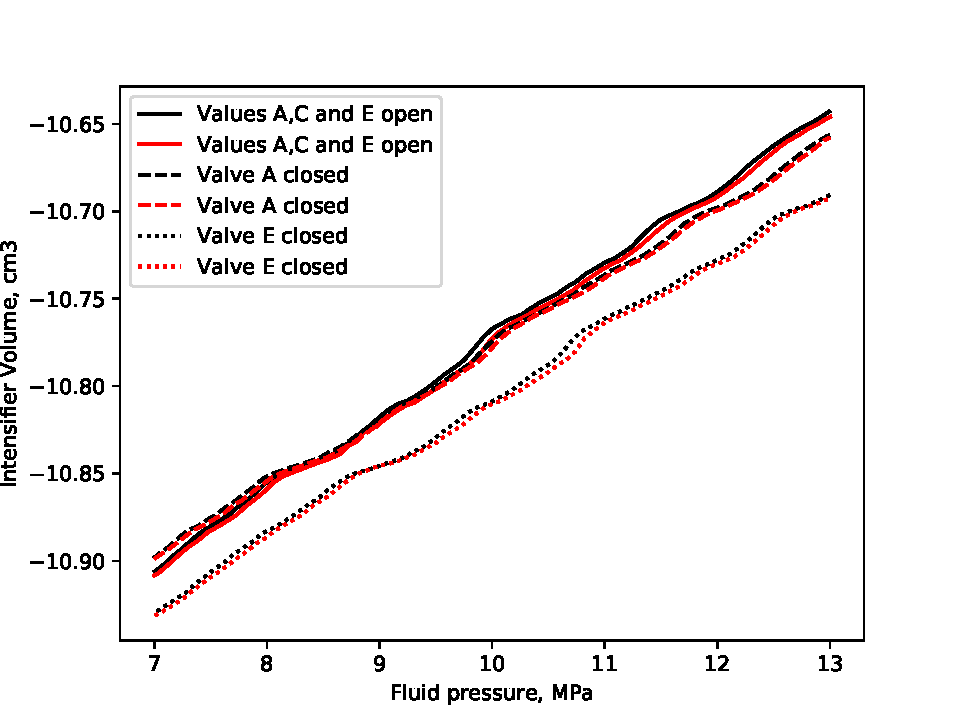
\includegraphics{figs/pfvol.pdf}
    \caption{PLACEHOLDER. The fluid volume change measured on the pore pressure intensifier due to controlled changes in fluid volume with a combination of valves open and closed.}
    \label{fig:pfcalib}
\end{figure}


\section{Modelling pore pressure diffusion}
\begin{itemize}
    \item Similar to section in my upgrade?
    \item Potentially some more detail of the equations in appendix
    \item At a minimum I need to describe the pore pressure diffusion equations and relevant boundary conditions for my experimental conditions.
    \item Show the solution to the relevant problems including plots of useful time series (log spaced) and parameters of importance (e.g. granite versus sandstone?)
    \item More details include the Laplace transform and solving for "poles" in the inverse Laplace transform.
\end{itemize}


The evolution of pore pressure in the sample over time can be modelled using the pore pressure diffusion equation, where 
\begin{equation}\label{eq:ppeqramp}
	\frac{\partial p}{\partial t} -\frac{k}{\beta_{\sigma} \mu}\frac{\partial^2 p}{\partial z^2} + \frac{B_i}{3} \frac{\partial \sigma_i}{\partial t},
\end{equation}
with initial condition
\begin{equation}
    p(z,t=0)=0,
\end{equation}
and boundary conditions
\begin{subequations}
\begin{equation}
    \left(\frac{\partial p }{\partial z}\right)_{z=0},
\end{equation}
\begin{equation}
    \beta_{\mathrm{res}}\left(\frac{\partial p }{\partial t}\right)_{z=L/2} +
    \frac{kA}{\mu}\left(\frac{\partial p }{\partial z}\right)_{z=L/2} = 0.
\end{equation}
\end{subequations}
We take an initially constant change in stress with time ($r$) followed by no change in stress after time $t_{\mathrm{end}}$,
%We assume that the change in stress with time is constant ($r$) until time $t_{\mathrm{end}}$, and then zero after:
\begin{equation}\label{eq:rampsource}
\frac{\partial \sigma_i}{\partial t} =
	\begin{cases}
		r, & 0< t \leq t_{\mathrm{end}},\\
		0, & t > t_{\mathrm{end}}.
	\end{cases}	
\end{equation}
We first normalise the system of equations using
\begin{subequations}
\begin{equation}
    t^* = t/ \tau,
\end{equation}
\begin{equation}
    z^* = z/L,
\end{equation}
\end{subequations}
where
\begin{equation}
    \tau = \frac{S_{\sigma}\mu L^2}{k}.
\end{equation}
Giving
\begin{subequations}
\begin{equation}
	\frac{\partial p}{\partial t^*} -\frac{\partial^2 p}{\partial {z^*}^2} =
	\begin{cases}
		\tau r, & 0< t^* \leq t_{\mathrm{end}}\tau =t_0,\\
		0, & t^* > t_{\mathrm{end}}\tau =t_0
	\end{cases},
\end{equation}
\begin{equation}
    p(z^*,t^*=0)=0,
\end{equation}
\begin{equation}
    \left(\frac{\partial p }{\partial z^*}\right)_{z^*=0},
\end{equation}
\begin{equation}
    \left(\frac{\partial p}{\partial t^*}\right)_{z^*=1/2} +
    h\left(\frac{\partial p}{\partial z^*}\right)_{z^*=1/2} = 0,
\end{equation}
\end{subequations}
where
\begin{equation}
    h = \frac{ALS_{\sigma}}{\beta_{\mathrm{res}}}.
\end{equation}
To solve this we apply the Laplace transform which is defined as (dropping the $^*$)
\begin{equation}
    \bar{p}(z,s) = \int_0^{\infty}e^{-st}p(z,t)dt,
\end{equation}
to get a new system of equations 
\begin{subequations}\label{eq:laplaceeqs}
\begin{equation}
	s\bar{p}(z,s) - \frac{\partial^2\bar{p}}{\partial z^2} =
	\begin{cases}
		\tau r \frac{1}{s}, & 0< t \leq t_0,\\
		\tau r \frac{1}{s} \left(1 - e^{-st_0}\right), & t > t_0
	\end{cases},
\end{equation}
\begin{equation}\label{eq:bc1}
    \left(\frac{\partial \bar{p} }{\partial z}\right)_{z=0} = 0,
\end{equation}
\begin{equation}\label{eq:bc2}
    s\bar{p}(z=1/2,s) +
    h\left(\frac{\partial p}{\partial z}\right)_{z=1/2} = 0.
\end{equation}
\end{subequations}
We solve equations \ref{eq:laplaceeqs} for $0< t \leq t_0$ and $t > t_0$ separately. First finding a particular solution for $t > t_0$
\begin{equation}
    \frac{\tau r}{s^2} \left( 1 - e^{-st_0} \right),
\end{equation}
and a solution to the homogeneous equation
\begin{equation}
    Ce^{-\sqrt{s}z} +De^{\sqrt{s}z},
\end{equation}
giving a general solution
\begin{equation}
   \bar{p} =  Ce^{-\sqrt{s}z} +De^{\sqrt{s}z} + \frac{\tau r}{s^2} \left( 1 - e^{-st_0} \right),
\end{equation}
where $C$ and $D$ are constants (in $z$) to be found. Using the boundary conditions from equation \ref{eq:bc1} and \ref{eq:bc2} and with some simplification gives
\begin{equation}\label{eq:Laplacesol}
    \bar{p} = \frac{\tau r \left( e^{-st_0} -1 \right)\left(\sqrt{s}\cosh{(\sqrt{s}z)} - \sqrt{s}\cosh{(\sqrt{s}/2)} -h\sinh{(\sqrt{s}/2)} \right)}{s^2\left(\sqrt{s}\cosh{(\sqrt{s}z)} - h\sinh{(\sqrt{s}/2)} \right)}.
\end{equation}
To find the solution the process of \cite{Hsieh1981}. The inverse Laplace transform is obtained using
\begin{equation}
    p(z,t) = \frac{1}{2\pi i}\int^{c+i\infty}_{c-i\infty}e^{st}\bar{p}(z,s)ds,\quad c \in \mathbb{R},
\end{equation}
where $s$ is complex and all the singularities lie within the contour left of the line $(c+i\infty,c-i\infty)$, with $c$ made large enough. The solution is given by the sum at the residues by Cauchy's residue theorem
\begin{equation}
    p(z,t) = \Sigma_m \mathrm{Res}(s_m),
\end{equation}
where $s_m$ are the poles of $e^{st}\bar{p}(z,s)$, and Res$(s_m)$ are the residues. There is a pole at $s=0$, and the residue is found by finding the Laurent series of the integrand and taking the coefficient of the order $z^{-1}$ term giving
\begin{equation}
    \mathrm{Res}(p,s=0) = \frac{\tau r t_0 h}{2+h}.
\end{equation}



%We get a solution to equation (\ref{eq:ppeqramp}) by applying a convolution of the solution given in equation (\ref{eq:ppsol}) with the ramp source term in equation (\ref{eq:rampsource}). Using the dimensional equation
%\begin{equation}
%\begin{split}
%	p(z,t) = \sum_{m=1}^{\infty}  \dfrac{2 \cos (2 \phi_{m} z/L) \sin (\phi_{m})}{\phi_{m} \cos (\phi_{m}) \sin (\phi_{m})}
%	\int_0^t e^{\frac{-4 \phi_{m}^{2}k}{\beta \mu L^2} (t-\lambda)}\frac{B_i}{3} \frac{\partial \sigma_i}{\partial \lambda}d\lambda\\
%- \dfrac{2}{h+2}\int_0^t  \frac{B_i}{3} \frac{\partial \sigma_i}{\partial \lambda}d\lambda
%+ \int_0^t H(t-\lambda) \frac{B_i}{3} \frac{\partial \sigma_i}{\partial \lambda}d\lambda.
%\end{split}
%\end{equation}
The solution has two parts, therefore pore pressure is expressed as
\begin{subequations}\label{eq:ppsolramp}
\begin{equation}\label{eq:ppsolrampa}
\begin{split}
	p(z,t) = \sum_{m=1}^{\infty}
	\dfrac{\cos (2 \phi_m z/L)e^{\frac{-4 \phi_{m}^{2}k}{\beta_{\sigma} \mu L^2} t} }{\phi_m^2\left((2+h)\cos (\phi_m) -\phi_m \sin (\phi_m)\right)}
	 \frac{\beta_{\sigma} \mu L^2}{k}\frac{B_i}{3}r\\
+ \dfrac{\left(6+h +12h(2+h)(\beta_{\sigma} \mu L^2/k)t -12(2+h)(z/L)^2\right)}{12(h+2)^2}\frac{\beta_{\sigma} \mu L^2}{k}  \frac{B_i}{3} r,
\end{split}
\end{equation}
for $0 < t \leq t_{\mathrm{end}}$ and
\begin{equation}\label{eq:ppsolrampb}
\begin{split}
	p(z,t) = \sum_{m=1}^{\infty} 
	\frac{\cos (2 \phi_m z/L)\left(e^{\frac{-4 \phi_{m}^{2}k}{\beta_{\sigma} \mu L^2} t} -
	e^{\frac{-4 \phi_{m}^{2}k}{\beta_{\sigma} \mu L^2} (t-t_0)} \right)}{\phi_m^2\left((2+h)\cos (\phi_m) -\phi_m \sin (\phi_m)\right)}
	\frac{\beta_{\sigma} \mu L^2}{k}\frac{B_i}{3}r \\
+ \frac{h}{h+2}\frac{\beta_{\sigma} \mu L^2}{k}  \frac{B_i}{3} r,
\end{split}
\end{equation}
\end{subequations}
for $t>t_{\mathrm{end}}$, where $z$ is normalised by the sample length $L$, $\phi_m$ are solutions of
\begin{equation}
2\phi +h\tan(\phi) =0,
\end{equation}
with
\begin{equation}
h = \frac{A\beta_{\sigma}L}{\beta_{\mathrm{res}}},
\end{equation}
$A$ is the cross-sectional area of the sample, and $\beta_{\mathrm{res}}$ is the storage of the reservoir at either end of the sample.

\section{Fitting pore pressure diffusion}
\begin{itemize}
    \item Details of procedure
    \item Inverse model for 3 parameters: $B_x$ (or $B_z$), $k$, and $\beta_{\sigma}$.
    \item Grid search to find least absolute difference between measurements and forward model.
\end{itemize}

\section{Development of method}
\begin{itemize}
    \item First experiment was not perfect and was build upon for experiment with data shown here.
    \item For example, piston friction was not properly considered and therefore small steps in applied axial load did not result in much change in load (and therefore stress) in the sample.
\end{itemize}

\section{Inversion of p and sh waves}
\subsection{group and phase velocity are not the same}
cite thomsen paper


\section{Description of experiment}
\subsection{Heat treatment}
The material used for this experiment was Westerly granite. A cylindrical sample, 40 mm in diameter and 100 mm in length was cored, with the ends ground flat and parallel to ensure parallelism within a precision of 0.02 mm. To generate open microcracks in the material, the sample was heat treated at room pressure to 600 $^{\circ}$C (past the $\alpha / \beta$ phase transition of quartz). The heating rate was 3 degrees C per minute, to minimise thermal gradients \citep{Wang2013}. The sample was left at 600 $^{\circ}$C for 3 hours, after which the temperature was decreased by 8 $^{\circ}$C per minute and then sample was left overnight to cool to room temperature. After thermal treatment, the sample expanded from an initial length of 100.00 mm to 100.90 mm and from a diameter of 40.08 mm to 40.40 mm.
\subsection{Bench top wave velocity measurements}

Wave velocity measurements were made at room  pressure in an intact sample of Westerly granite and in the same sample following thermal treatment to a maximum of 600 $^\circ$C. In the intact sample p-wave velocity was 4.9 km/s vertically and 5.2 km/s horizontally, and s-wave velocity was 2.8 km/s vertically and 2.7 km/s horizontally. After heating, p-wave velocity was 1.1 km/s vertically and 1.4 km/s horizontally, and s-wave velocity was 0.7 km/s vertically and 0.8 km/s horizontally.

\chapter{Stress-induced anisotropic poroelasticity in granite}
\label{chapterlabel3}

Paper transferred into thesis format.

\section{Maybe add in some data from the saturated wave velocities? Have I processed these?}


\chapter{The poroelastic response of cracked Westerly granite to cyclical changes in load}
\chapter{Discussion}
\chapter{Conclusions and future work}


\phantomsection
\addcontentsline{toc}{chapter}{Appendices}

% The \appendix command resets the chapter counter, and changes the chapter numbering scheme to capital letters.
%\chapter{Appendices}
\appendix
\chapter{An Appendix About Stuff}
\label{appendixlabel1}
(stuff)

\chapter{Another Appendix About Things}
\label{appendixlabel2}
(things)

\chapter{Colophon}
\label{appendixlabel3}
\textit{This is a description of the tools you used to make your thesis. It helps people make future documents, reminds you, and looks good.}

\textit{(example)} This document was set in the Times Roman typeface using \LaTeX\ and Bib\TeX , composed with a text editor. 
 % description of document, e.g. type faces, TeX used, TeXmaker, packages and things used for figures. Like a computational details section.
% e.g. http://tex.stackexchange.com/questions/63468/what-is-best-way-to-mention-that-a-document-has-been-typeset-with-tex#63503

% Side note:
%http://tex.stackexchange.com/questions/1319/showcase-of-beautiful-typography-done-in-tex-friends
 
% You could separate these out into different files if you have
%  particularly large appendices.

% Actually generates your bibliography. The fact that \include is 
% the last thing before this ensures that it is on a clear page.
\bibliography{Bibliography}

% All done. \o/
\end{document}
